\appendix
\pagenumbering{Roman}
\section{Appendix}
\subsection{Sensitivity}
\label{A:sensitivity}
In this section we examine the sensitivity of our model with respect to certain parameters. We use 10-start multi-start optimizations for the Pareto optimal and the unrestricted strategy. We use 10 starts instead of 50, as in the main section, to reduce the computational costs. The results should therefore not be compared to the results from the main section regarding to absolute numbers. However, we can use the results of the sensitivity analysis to learn about the influence of parameter changes on the death cases.

\subsubsection{Sensitivity of cross-border enocunters}
\label{A:encounters}
In Figure \ref{fig:sensitivity}, we examine the influence of the parameter that determine cross-border encounters on the number of deaths. Recall that the distance function $b(d(A,B))$ maps to the unit interval and $b$ is strictly decreasing such that large distances between countries result in fewer cross-border encounters. From Equation \eqref{eq:cond_meeting_prob}, we have derived that $b(d(A,B)) \to 1$ means that cross-border encounters are equally likely as within-country encounters and that $b(d(A,B)) \to 0$ means that cross-border encounters become unlikely.
\begin{figure}[h!]
\centering
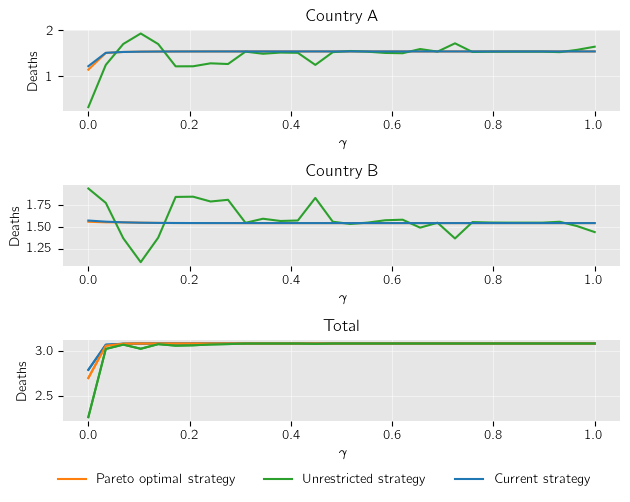
\includegraphics[scale=0.59]{images/sensitivity.png}
\begin{flushleft}
\scriptsize{Note:} To compute the optimized values of the Pareto strategy and the unrestricted strategy a multi-start with 10 runs has been conducted.
\end{flushleft}
\caption{Sensitivity with respect to the distance measure}
\label{fig:sensitivity}
\end{figure}

We see as major takeaway from Figure \ref{fig:sensitivity} that the optimal strategies only outperform the current strategy for low values of $b(d(A,B))$. This could indicate that no improvement is possible, if cross-border encounters happen frequently. This might be explained by the fact that for high values of $b(d(A,B))$, individuals are likely to become infected from individuals of both countries such that the allocation of a fixed amount of vaccine doses cannot protect a certain country. This seems plausible and we see it as a proof of concept. However, simulations using more multi-starts might be necessary to fully examine the patterns.

%We observe for country A that there is a steep increase in the death cases if we increase the distance function for all three strategies. This can be attributed to increased case numbers of the mutant type in country A, which is only present in country B at the beginning but spills over further for high values of $b(d(A,B))$. However, this increase saturates fast and seems to converge to a maximum. This could be the point where only the mutant spreads and, thus, a lower distance has almost no influence on the death cases anymore. In line with the findings for country A are the results for country B. Since the wild-type spreads more in country B for high $b(d(A,B))$ as for low values, the numbers decrease. However, the decrease is not as steep as the increase in country A.  

%The sum of both countries yields a steep increase up to around $b(d(A,B))=0.2$. For $b(d(A,B))>0.2$ it seems that all strategies yield the same number of deaths such that no improvement is possible by optimizing vaccination strategies. Heuristically, at this point influence cross-country infections the pandemic that much such that vaccine allocations of the fixed amount of available vaccine doses do not change the results.

\subsubsection{Sensitivity of the mutant infectiousness}
\label{A:eta}

We trace out the effect of the infectiousness of the mutant type in Figure \ref{fig:sensitivity_eta}. As expected, the number of deaths increases with a more infectious mutant. Most strikingly, it seems that there is only a corridor around the interval $\eta \in [1.15, 1.4]$ where a Pareto improvement is possible. We hypothesize that for $\eta \in [1, 1.15)$ the effect of the higher mutant-infectiousness is negligible and for $\eta \in (1.4, 2]$ the effect is too severe, such that both countries experience a similar amount of deaths which cannot be influenced by the vaccine allocation. The latter is enhanced by the finding that for high values of $\eta$, country A and country B have similar numbers of deaths for the Pareto and the current strategy.
\begin{figure}[h!]
\centering
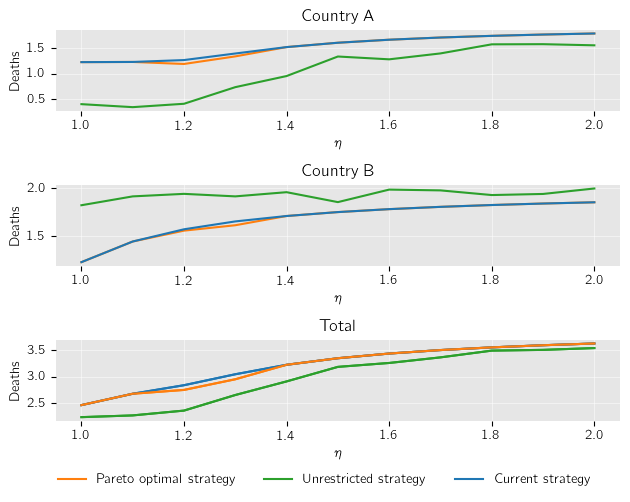
\includegraphics[scale=0.59]{images/sensitivity_eta.png}
\begin{flushleft}
\scriptsize{Note:} To compute the optimized values of the Pareto strategy and the unrestricted strategy a multi-start with 10 runs has been conducted.
\end{flushleft}
\caption{Sensitivity with respect to the parameter $\eta$}
\label{fig:sensitivity_eta}
\end{figure}



\subsubsection{Sensitivity of virus spread prevention by vaccines}
\label{A:gamma}
In Figure \ref{fig:sensitivity_gamma}, we depict the sensitivity of number of deaths with respect to the parameter $\gamma$. Recall that $\gamma$ is the reduction of transmitting the virus if an individual is vaccinated. 

We find that the order of the strategies does not change over the whole range of $\gamma$. The number of death cases decreases nearly linear for the Pareto optimal and the current strategy but the decrease is rather small. This might be explained by the small number of individuals that become infected if they are vaccinated such that the influence of the not transmitting the virus does not influence the model severely. For the unrestricted optimal strategy, we observe peeks which could occur by chance due to the random draws of the starting values for the optimization. However, further research is needed to fully answer why these peeks occur.


\begin{figure}[h!]
\centering
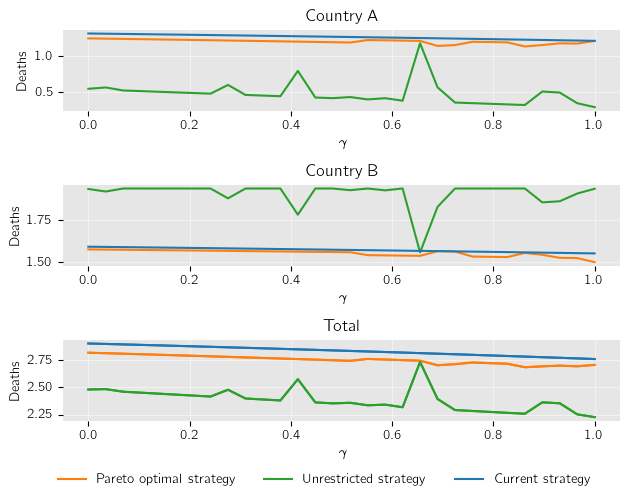
\includegraphics[scale=0.59]{images/sensitivity_gamma.png}
\begin{flushleft}
\scriptsize{Note:} To compute the optimized values of the Pareto strategy and the unrestricted strategy a multi-start with 10 runs has been conducted.
\end{flushleft}
\caption{Sensitivity with respect to the parameter $\gamma$}
\label{fig:sensitivity_gamma}
\end{figure}


\clearpage


\subsection{Supplementary results}
We plot Figures that enhance our line of argumentation but would disturb the train of reading within the main section.
\subsubsection{Piecewise constant results}
\label{A:piecewise}
Figure \ref{fig:results_piecewise_numbers} provides a visualization of the core results using piecewise constant vaccination channels as functional form of $f_l$. The values do qualitatively not differ from the corresponding spline values depicted in the main text in Figure \ref{fig:results_splines_numbers}. Even the percentage improvements of the unrestricted and the Pareto strategy equal the numbers from the spline analysis. Since the current strategy is not affected by the type of the vaccination channel, it yields the exact same results as in Figure \ref{fig:results_splines_numbers}. For the optimized strategies, numbers are slightly shifted between countries, such that country A experiences between 10,000-30,000 more and country B fewer deaths. 
\begin{figure}[h!]
\centering
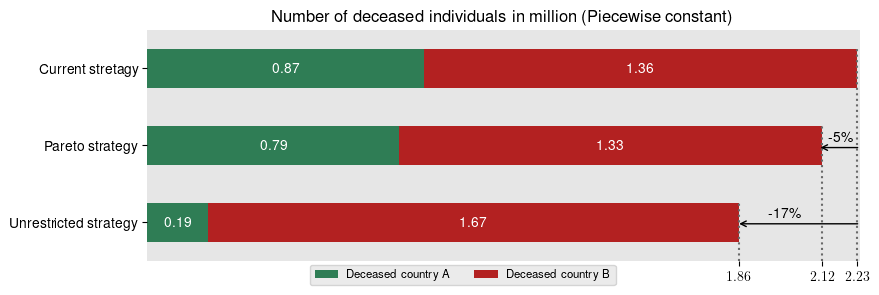
\includegraphics[scale=0.65]{images/piecewise_percentage_deviation.png}
\begin{flushleft}
\scriptsize{Note: The numbers within the boxes indicate the number of deceased individuals in millions with respect to the respective country and strategy. Numbers at the x-axis represent the total number of deceased individuals within one country. The percentage numbers indicate the change relative to the optimal strategy, e.g. $-5\%$ indicates that by implementing the Pareto strategy 5\% less individuals died in comparison to the current strategy.}
\end{flushleft}
\caption{Number of deceased individuals by country (stepwise)}
\label{fig:results_piecewise_numbers}
\end{figure}
Figure \ref{fig:results_piecewise_allocation} depicts the optimal doses of vaccine inflow using piecewise constant vaccination channels as functional form of $f_l$. As for the number of deceased individuals, the values do qualitatively not differ from the corresponding spline values depicted in the main text in Figure \ref{fig:results_splines_allocation}. Especially, we observe the pattern for the unrestricted strategy, which only assigns vaccine doses to country B between week 5 to 9. %However, the peak is not as large as in Figure \ref{fig:results_splines_allocation}. As opposed to Figure \ref{fig:results_splines_allocation}, there is no allocation of vaccines to country B at the very beginning, which could explain the higher number of death cases in country B using the stepwise vaccination channel. \\

\begin{figure}[h!]
\centering
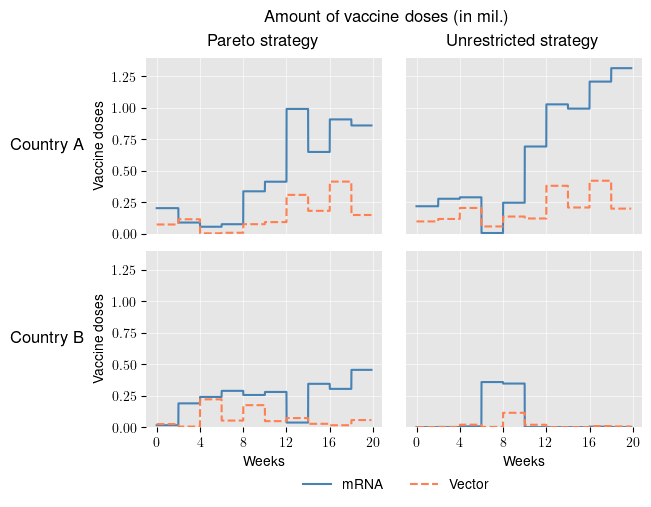
\includegraphics[scale=0.6]{images/piecewise_vaccine_total_quantity.png}
\begin{flushleft}
\scriptsize{Note:} Every column represents one vaccination strategy and every row represents one country. Both vaccines are indicated by their colors that are used throughout the paper. 
Every curve is the product of a piecewise constant vaccine inflow and a spline. Thus, the lines appear to be discontinuous piecewise polynomials. 
\end{flushleft}
\caption{Number of allocated vaccine doses (stepwise)}
\label{fig:results_piecewise_allocation}
\end{figure}
In Figure \ref{fig:results_piecewise_infectious_dead}, we trace out the trajectories of the number of infectious and deceased individuals according to the respective strategies (columns) and countries (rows). The values do not qualitatively differ form the corresponding spline values depicted in the main text in Figure \ref{fig:results_splines_infectious_dead}.\\

\begin{figure}[h!]
\centering
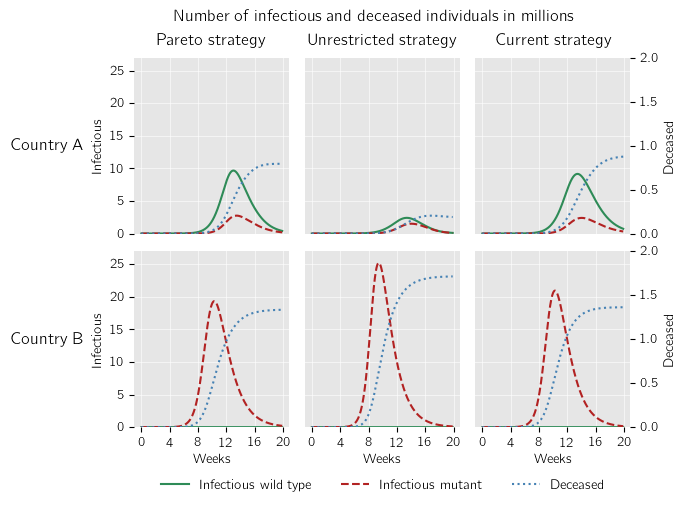
\includegraphics[scale=0.6]{images/piecewise_infectious_dead.png}\\
\begin{flushleft}
\scriptsize{Note:} Every column represents one vaccination strategy and every row represents one country. Every vaccine is indicated by its color that is used throughout the paper. The left y-axis is used for the number of infectious individuals (solid green and dashed red curves). The right y-axis corresponds to the number of deceased individuals (dotted blue line). Both viruses are associated with the color we have used throughout the paper. 
\end{flushleft}
\caption{Number of infectious individuals (stepwise)}
\label{fig:results_piecewise_infectious_dead}
\end{figure}

\clearpage
\subsubsection{Vaccination allocation fractions}
\label{A:fractions}

Figure \ref{fig:results_piecewise_allocation_fractions} depicts the course of $f_l$ over the whole decison period using a piecewise vaccination channel. Figure \ref{fig:results_splines_allocation_fractions} shows the respective values for the spline vaccination channels. The values are the quotient of the curve of the vaccine inflow in Figure \ref{fig:available_vaccine} and the optimal total number of vaccine doses inflow in Figure \ref{fig:results_piecewise_allocation} and Figure \ref{fig:results_splines_allocation}. The current strategy allocates half of the available vaccine doses to each country.
\begin{figure}[h!]
\centering
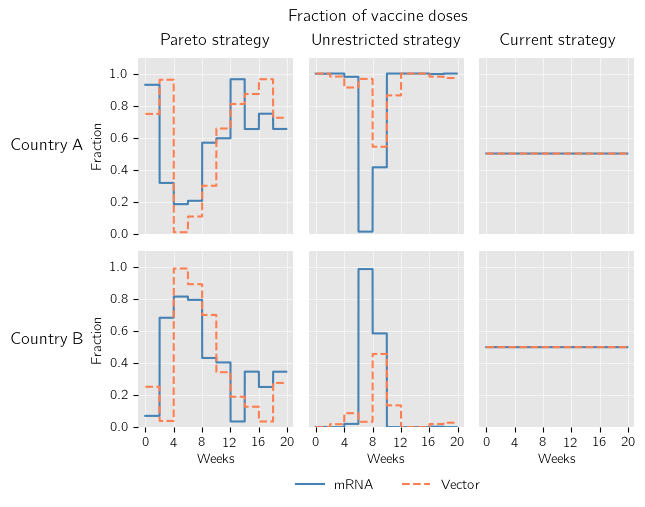
\includegraphics[scale=0.75]{images/piecewise_vaccine_fractions.png}\\
\begin{flushleft}
\scriptsize{Note:} Every column represents one vaccination strategy and every row represents one country. Both vaccines are indicated by their colors that are used throughout the paper. 
\end{flushleft}
\caption{Fractions of vaccines (stepwise)}
\label{fig:results_piecewise_allocation_fractions}
\end{figure}

\begin{figure}[h!]
\centering
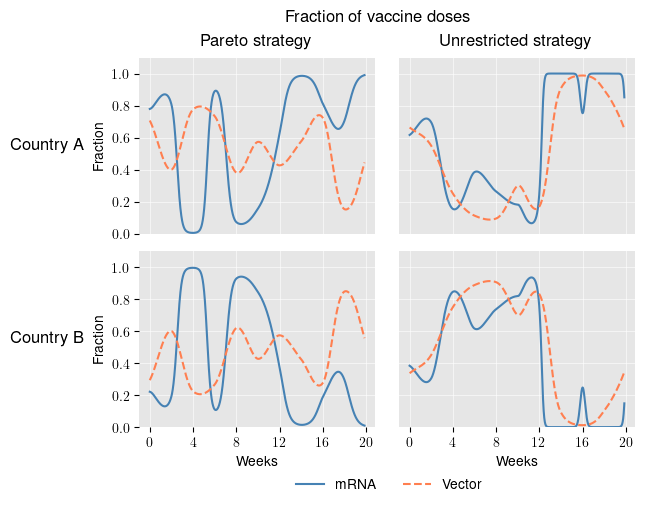
\includegraphics[scale=0.75]{images/splines_vaccine_fractions.png}\\
\begin{flushleft}
\scriptsize{Note:} Every column represents one vaccination strategy and every row represents one country. Both vaccines are indicated by their colors that are used throughout the paper. 
\end{flushleft}
\caption{Fractions of vaccines (splines)}
\label{fig:results_splines_allocation_fractions}
\end{figure}

\clearpage
\subsubsection{Waterfall plots of optimization}
\label{A:waterfall}

Figure \ref{fig:results_piecewise_waterfall} and Figure \ref{fig:results_splines_waterfall} show the ordered 20 multi-start runs with the lowest optima of all 50 runs. We only show 20 runs to increase readability of the plot. We find that the descend of the ordered function values does not contain many jumps and the optimal values are obtained only once. Hence, it might be possible to find even lower values using more multi-start runs.


\begin{figure}[h!]
     \centering
     \begin{subfigure}[b]{0.49\textwidth}
	\centering
	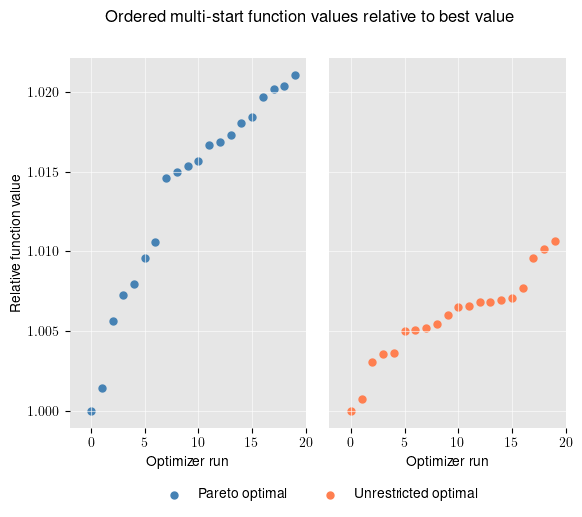
\includegraphics[scale=0.5]{images/piecewise_waterfall.png}

	\caption{Stepwise}
	\label{fig:results_piecewise_waterfall}
     \end{subfigure}
     \hfill
     \begin{subfigure}[b]{0.49\textwidth}
	\centering
	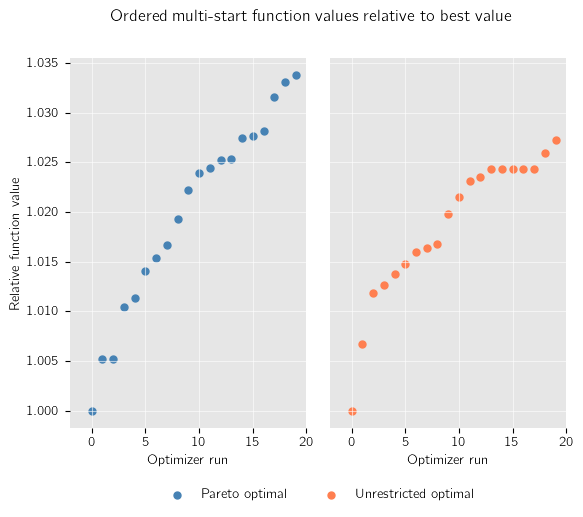
\includegraphics[scale=0.5]{images/splines_waterfall.png}
	\caption{Splines}
	\label{fig:results_splines_waterfall}
     \end{subfigure}
\begin{flushleft}
\scriptsize{Note:} Values are relative to the start yielding the lowest optimal minimum value. Only 	the best 20 starts are used to increase readability. 
\end{flushleft}
        \caption{Waterfall plot of the 20 best multi-start runs (splines)}
        \label{fig:histograms} 
\end{figure}






\clearpage
\subsubsection{Simulated distribution of number of deceased individuals}
\label{A:simulated_distr}

Figure \ref{fig:results_piecewise_stochastic_histogram} depicts the results for the number of deceased individuals using piecewise constant vaccination channels. We decided to remove it from the main text since the results resemble the results from the spline vaccination channel in Figure \ref{fig:results_splines_stochastic_histogram} in the main section.
\begin{figure}[h!]
\centering
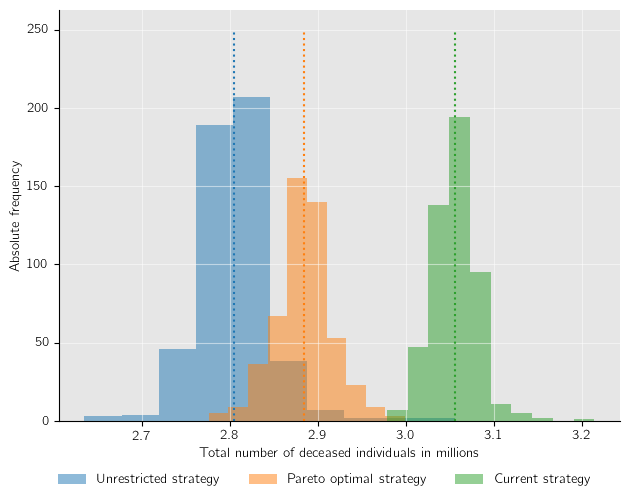
\includegraphics[scale=0.65]{images/piecewise_stochastic_histogram.png}\\
\begin{flushleft}
\scriptsize{Note:} Dotted lines are sample means. The total number of deceased individuals of a strategy is the sum of the respective number of deaths in in country A and country B. We draw 500 samples per strategy. 
\end{flushleft}
\caption{Stochastically observed frequencies (stepwise)}
\label{fig:results_piecewise_stochastic_histogram}
\end{figure}

Figure \ref{fig:results_piecewise_infectious_dead_stochastic} plots the total number of infectious individuals simulated using the stochastic model. We decided to remove it from the main text since the results resemble the results from the spline vaccination channel within Figure \ref{fig:results_splines_infectious_dead_stochastic} in the main section.\\

\begin{figure}[h!]
\centering
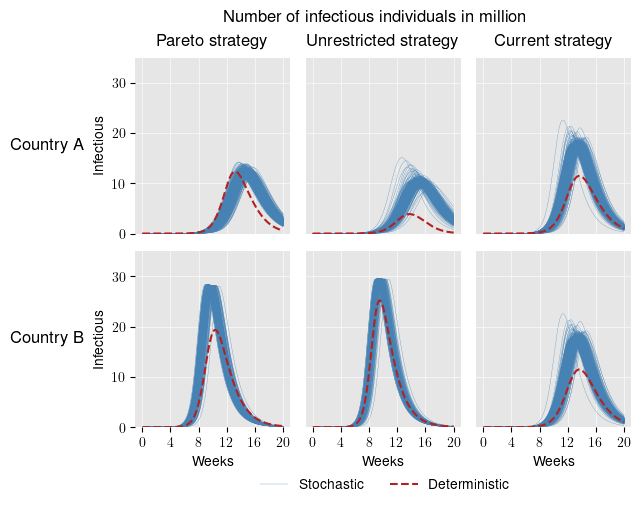
\includegraphics[scale=0.75]{images/piecewise_stochastic_infectious.png}\\
\begin{flushleft}
\scriptsize{Note:} Every column represents one vaccination strategy and every row represents one country. The thin blue lines depict all 500 simulations of the stochastic algorithm using the respective strategy. The dashed red depicts the respective infections within the deterministic model. 
\end{flushleft}
\caption{Number of infectious individuals using stochastic simulations (stepwise)}
\label{fig:results_piecewise_infectious_dead_stochastic}
\end{figure}
\newpage
Figures \ref{fig:histograms}  and \ref{fig:histograms_piecewise} depict the 2-dimensional, as well as the marginal, histograms of the number of deceased individuals with respect to the countries. As for the results shown within the main section, the results are qualitatively highly similar. It is striking that for the unrestricted case, the case with the fewest deaths, points seem to fluctuate more random around the center point mass than for the Pareto optimal and the current strategy. For the current strategy and the optimal strategy the reasoning might be that, just by chance, some simulated pandemics result in overall more deaths and therefore both countries have increased numbers in death cases. However, the same reasoning could apply for the unrestricted strategy that shows no linear correlation.
Further research is needed to examine if this patterns occurred randomly.
\begin{figure}[h!]
     \centering
     \begin{subfigure}[b]{0.49\textwidth}
         \centering
         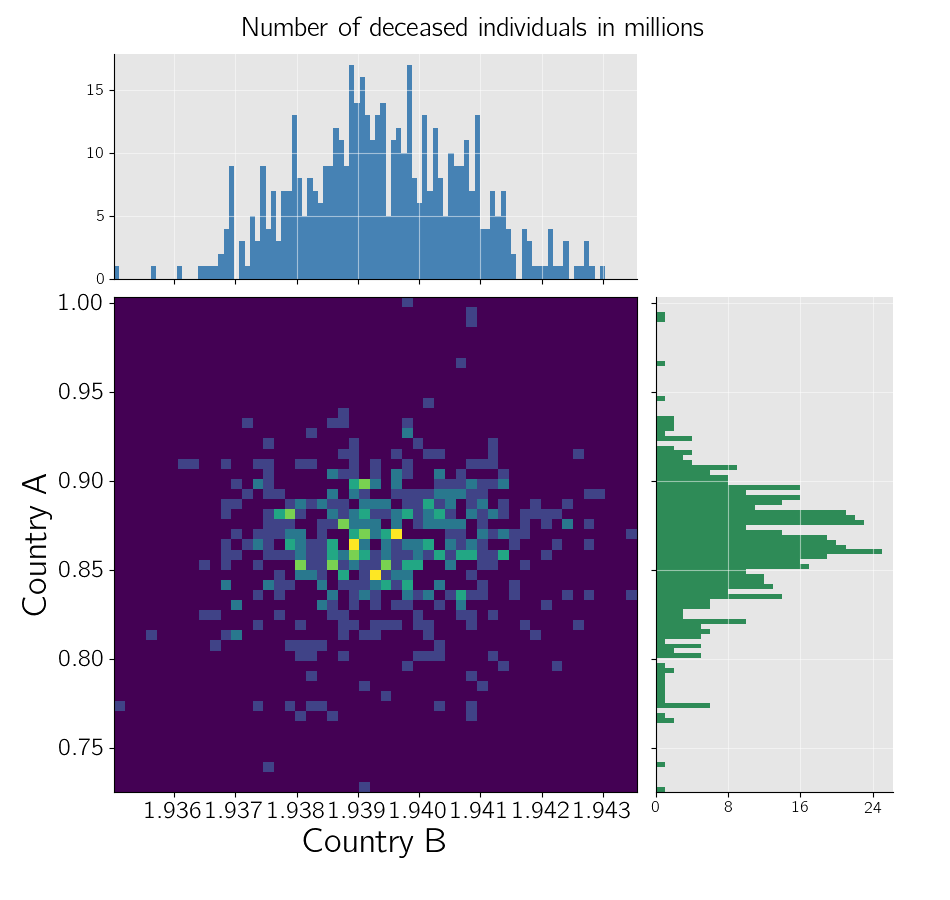
\includegraphics[width=\textwidth]{images/splines_stochastic_histogram_deceased_unrestricted.png}
         \caption{Unrestricted strategy}
         \label{fig:2d_unrestricted}
     \end{subfigure}
     \hfill
     \begin{subfigure}[b]{0.49\textwidth}
         \centering
         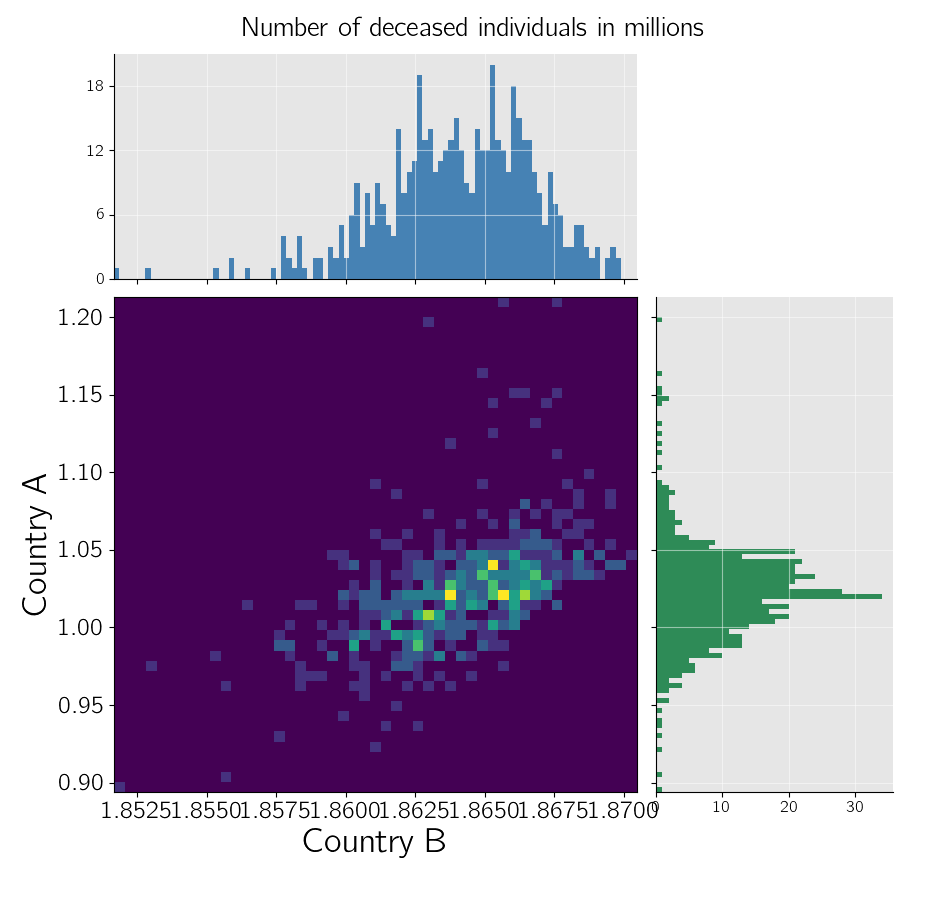
\includegraphics[width=\textwidth]{images/splines_stochastic_histogram_deceased_optimal.png}
         \caption{Pareto optimal strategy}
         \label{fig:2d_optimal}
     \end{subfigure}
     \\
     \begin{subfigure}[b]{0.49\textwidth}
         \centering
         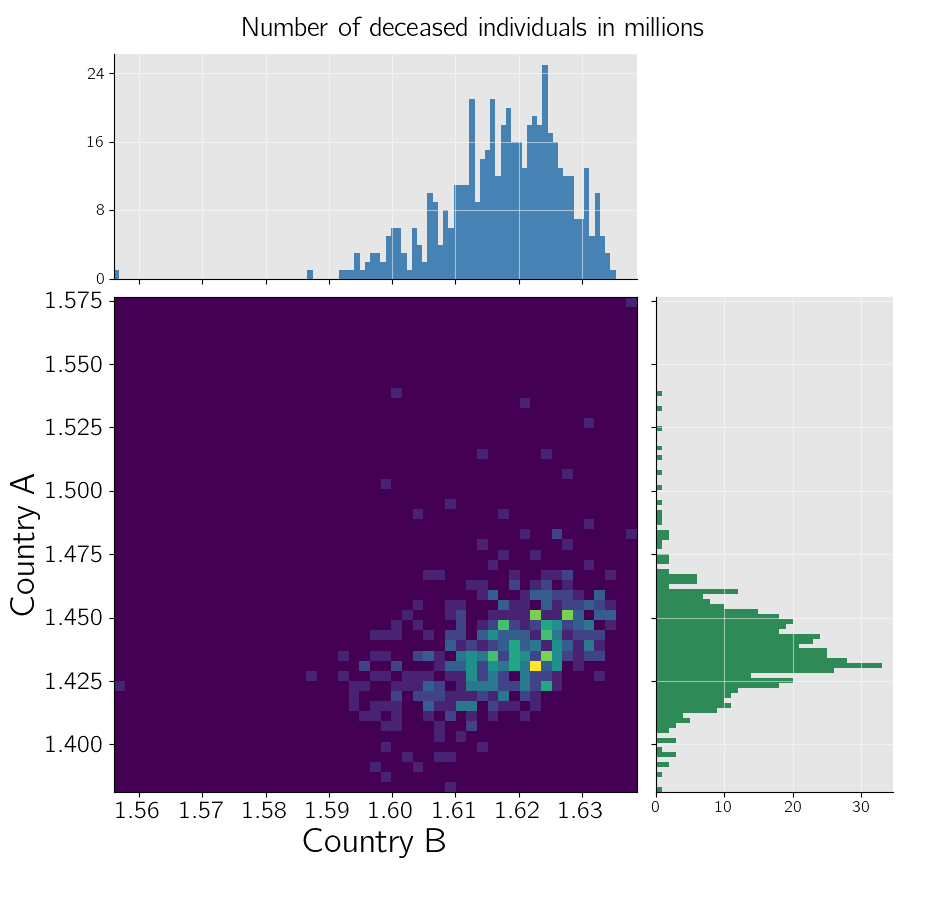
\includegraphics[width=\textwidth]{images/splines_stochastic_histogram_deceased_current.png}
         \caption{Current strategy}
         \label{fig:2d_current}
     \end{subfigure}
\begin{flushleft}
\scriptsize{Note:} Purple temperature boxes indicate the joint frequencies. Histograms on top are the histograms corresponding to country B and histograms at the right-hand side are the histograms corresponding to country A. Histograms are computed using 500 simulations of the stochastic model using the Policies derived from splines. 
\end{flushleft}
        \caption{Frequencies of number of deceased individuals (splines)}
        \label{fig:histograms} 
\end{figure}

\begin{figure}[h!]
     \centering
     \begin{subfigure}[b]{0.49\textwidth}
         \centering
         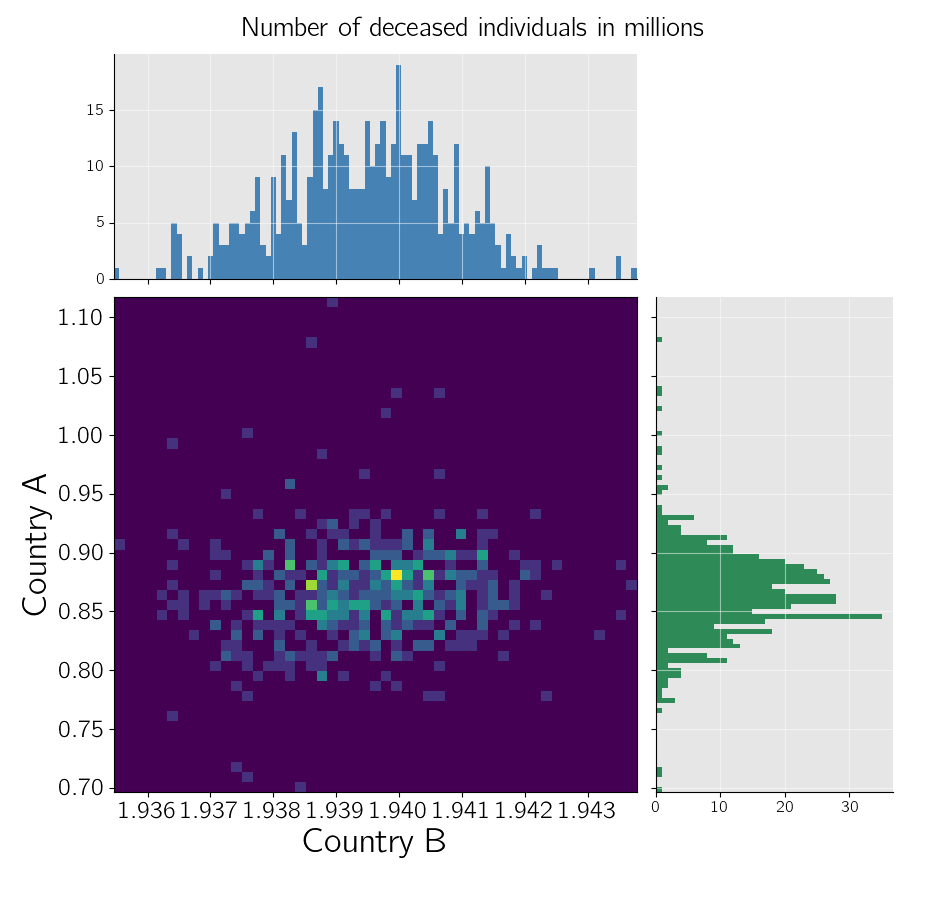
\includegraphics[width=\textwidth]{images/piecewise_stochastic_histogram_deceased_unrestricted.png}
         \caption{Unrestricted strategy}
         \label{fig:2d_unrestricted_piecewise}
     \end{subfigure}
     \hfill
     \begin{subfigure}[b]{0.49\textwidth}
         \centering
         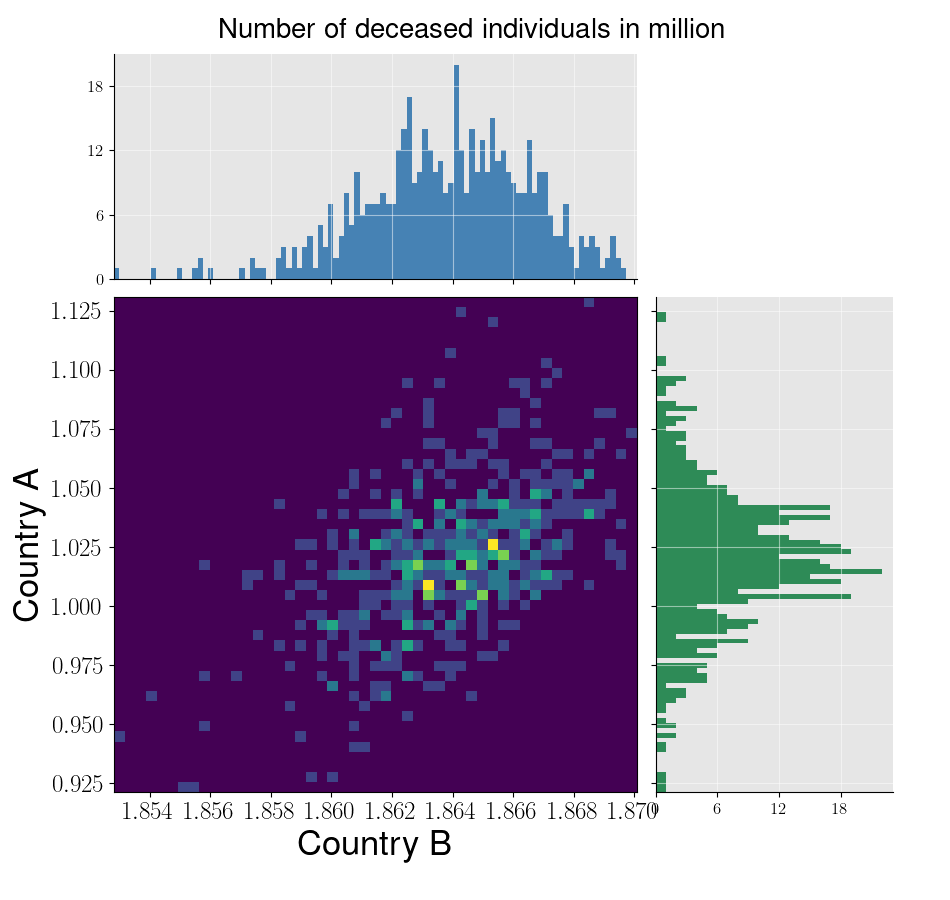
\includegraphics[width=\textwidth]{images/piecewise_stochastic_histogram_deceased_optimal.png}
         \caption{Pareto optimal strategy}
         \label{fig:2d_optimal_piecewise}
     \end{subfigure}
     \\
     \begin{subfigure}[b]{0.49\textwidth}
         \centering
         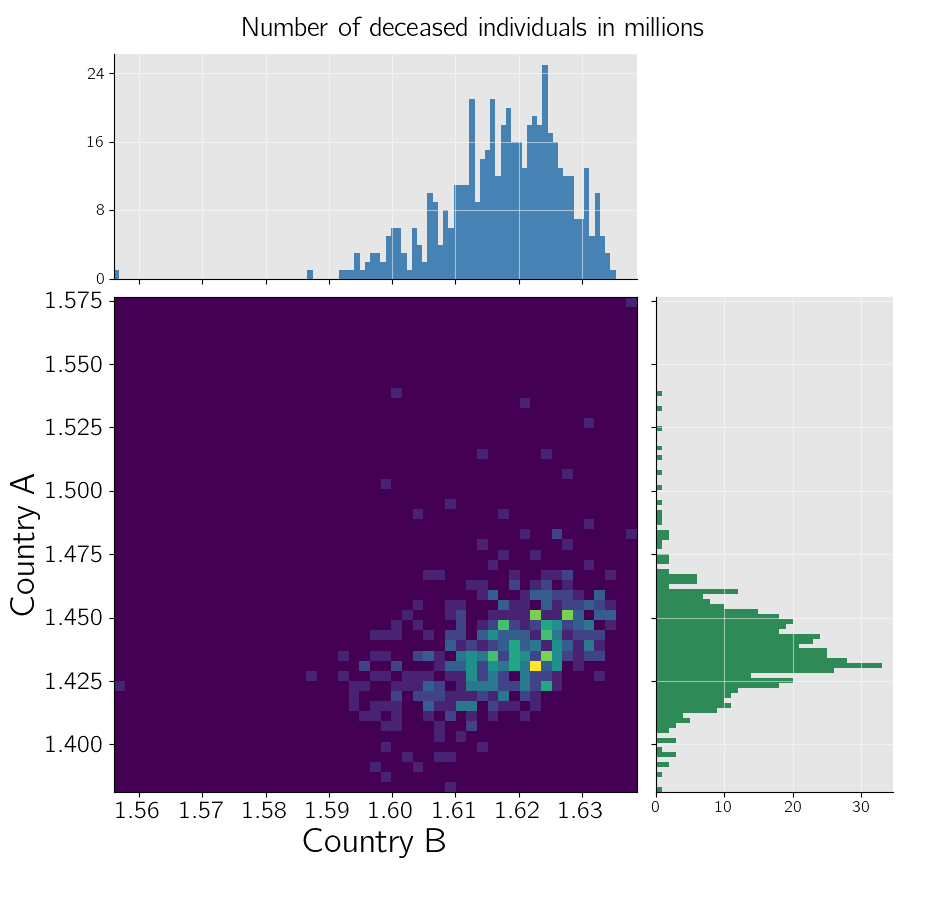
\includegraphics[width=\textwidth]{images/piecewise_stochastic_histogram_deceased_current.png}
         \caption{Current strategy}
         \label{fig:2d_piecewise}
     \end{subfigure}
\begin{flushleft}
\scriptsize{Note:} Purple temperature boxes indicate the joint frequencies. Histograms on top are the histograms corresponding to country B and histograms at the right-hand side are the histograms corresponding to country A. Histograms are computed using 500 simulations of the stochastic model using the Policies derived from splines. 
\end{flushleft}
        \caption{Frequencies of number of deceased individuals (stepwise)}
        \label{fig:histograms_piecewise} 
\end{figure}

\clearpage

\subsection{Calculations and proofs}
We provide calculations and proofs that enhance our line of argumentation but would disturb the train of reading within the main section.
\subsubsection{Encounter probabilities}
\label{A:meeting_prob}
Using Bayes formula, we can rewrite the conditional probability as follows
\begin{align}
\label{eq:cond_meeting_prob}
&\quad \   \prob_t(i_2 \in \set(X_S, C_j, F_2)|i_1 \in \set(\neg X_D, C_A)) \\ &= \prob_t(i_2 \in \set(\neg X_D, C_j, F_2) | i_1 \in \set(\neg X_D, C_A) )  \notag \\
& \quad \cdot \prob_t(i_2 \in \set(X_S) | i_1 \in \set(\neg X_D, C_A), i_2 \in \set(\neg X_D, C_j, F_2) ) \notag \\
&= \prob_t(i_2 \in \set(\neg X_D, C_j, F_2) | i_1 \in \set(\neg X_D, C_A) )  \notag \\
& \quad \cdot \prob_t(i_2 \in \set(X_S)|i_2 \in \set(\neg X_D, C_j, F_2)  \notag
\end{align} 
We use the relative number of susceptible individuals $\set(X_S, C_j, F_2)$ across all individuals of $\set(\neg X_D, C_j, F_2)$ as approximation of the probability at the second line of the right-hand side 
\begin{align}
 \prob_t(i_2 \in \set(X_S, F_2)|i_2 \in \set(\neg X_D, C_j, F_2) ) = \frac{\num(X_S, C_j, F_2)}{\num(\neg X_D, C_j, F_2)}.
\end{align}

To account for the origin of $i_1$ within the first line of the right hand-side, we distinguish between the cases where $i_2 \in \set(C_A)$ and $i_2 \in \set(C_B)$. Assume that $i_2 \in \set(X_S, C_B, F_2)$. If there were no spatial effects to influence the cross-border encounter frequency we would use the unconditional probability 
\begin{align}
\prob_t(i_2 \in \set(\neg X_D, C_j, F_2)) = \frac{\num(\neg X_D, C_j, F_2)}{ \num(\neg X_D)}.   
\end{align}
To account for the spatial effects, we introduce a penalty function $b: \R_+ \to [0,1]$ that depends on the distances between both countries $d(A, B)$
\begin{align}
\label{eq:prob_cross_border}
\prob_t(i_2 \in \set(\neg X_D, C_B, F_2) | i_1 \in \set(\neg X_D, C_A) ) = \prob_t\left(i_2 \in \set(\neg X_D, C_B, F_2)\right) \cdot b(d(A, B)),
\end{align}
yielding
\begin{align}
\label{eq:cond_meeting_prob_b}
\prob_t(i_2 \in \set(X_S, C_B, F_2)|i_1 \in \set(\neg X_D, C_A)) &= \frac{\num(X_S, C_j, F_2)}{\num(\neg X_D)} \cdot b(d(A, B))
\end{align} 


\subsubsection{Well-conditioning of the polynomial basis}
\label{A:well_conditioning}
The basis polynomials are defined by $B_1(t) = 2t^3 - 3t^2 +1, B_2(t) = t^3 - 2t^2 +t, B_3(t) = -2t^3 + 3t^2$ and $B_4(t) = t^3 - t^2$. First note that $B_1(0) = 1$ and $B_2(0), B_3(0), B_4(0) = 0$. Furthermore, $B_1(1), B_2(1), B_4(1) = 0$ and $B_3(1) = 1$. We first compute the function values at the boundaries $t_{i-1}$ and $t_i$.
\begin{align*}
P_{l,i}(t_{i-1}) &= B_1(0) P_{l,i}(t_{i-1}) + B_2(0) (t_{i} - t_{i-1}) P'_{l,i}(t_{i-1})  \\& \quad + B_3(0) P_{l,i}(t_{i}) + B_4(0) (t_{i} - t_{i-1}) P'_{l,i}(t_{i}) \\
&=  1 \cdot P_{l,i}(t_{i-1}) + 0 \cdot (t_{i} - t_{i-1}) P'_{l,i}(t_{i-1})  \\& \quad + 0 \cdot P_{l,i}(t_{i}) + 0 \cdot (t_{i} - t_{i-1}) P'_{l,i}(t_{i})\\
&= P_{l,i}(t_{i-1}) 
\end{align*}
\begin{align*}
P_{l,i}(t_{i}) &= B_1(1) P_{l,i}(t_{i-1}) + B_2(1) (t_{i} - t_{i-1}) P'_{l,i}(t_{i-1})  \\& \quad + B_3(1) P_{l,i}(t_{i}) + B_4(1) (t_{i} - t_{i-1}) P'_{l,i}(t_{i}) \\ 
&= 0 \cdot P_{l,i}(t_{i-1}) + 0 \cdot (t_{i} - t_{i-1}) P'_{l,i}(t_{i-1})  \\& \quad + 1 \cdot  P_{l,i}(t_{i}) + 0 \cdot (t_{i} - t_{i-1}) P'_{l,i}(t_{i})  \\
&= P_{l,i}(t_{i})
\end{align*}

The derivatives of the basis polynomials are 
\begin{align*}
B_1'(t) &= 6t^2 - 6t \\
B_2'(t) &= 3t^2 - 4t + 1 \\
B_3'(t) &= -6t^2 + 6t \\
B_4'(t) &= 3t^2 - 2t
\end{align*}
with $B_1(0)'=B_3(0)'=B_4(0)'=0$ and $B_2(t)'=\frac{1}{t_i - t_{i-1}}$. Moreover, $B_1'(1)'= B_2(1)'=B_3(1)'=0$ and $B_4(1)'=\frac{1}{t_i - t_{i-1}}$. The derivative of the polynomial is simply
\begin{align*}
P_{l,i}'(t) &= B_1'(t') P_{l,i}(t_{i-1}) + B_2'(t') (t_{i} - t_{i-1}) P'_{l,i}(t_{i-1})  \\& \quad + B_3'(t') P_{l,i}(t_{i}) + B_4'(t') (t_{i} - t_{i-1}) P'_{l,i}(t_{i})
\end{align*}
and therefore
\begin{align*}
P_{l,i}'(t_{i-1}) &= B_1'(0) P_{l,i}(t_{i-1}) + B_2'(0) (t_{i} - t_{i-1}) P'_{l,i}(t_{i-1})  \\& \quad + B_3'(0) P_{l,i}(t_{i}) + B_4'(0) (t_{i} - t_{i-1}) P'_{l,i}(t_{i}) \\
&= 0 \cdot P_{l,i}(t_{i-1}) + \frac{1}{t_i - t_{i-1}} \cdot(t_{i} - t_{i-1}) P'_{l,i}(t_{i-1})  \\& \quad + 0 \cdot P_{l,i}(t_{i}) + 0 \cdot (t_{i} - t_{i-1}) P'_{l,i}(t_{i}) \\
&=  P'_{l,i}(t_{i-1})
\end{align*}
and 
\begin{align*}
P_{l,i}'(t_{i-1}) &= B_1'(1) P_{l,i}(t_{i-1}) + B_2'(1) (t_{i} - t_{i-1}) P'_{l,i}(t_{i-1})  \\& \quad + B_3'(1) P_{l,i}(t_{i}) + B_4'(1) (t_{i} - t_{i-1}) P'_{l,i}(t_{i}) \\
&= 0 \cdot P_{l,i}(t_{i-1}) + 0 \cdot(t_{i} - t_{i-1}) P'_{l,i}(t_{i-1})  \\& \quad + 0 \cdot P_{l,i}(t_{i}) + \frac{1}{t_i - t_{i-1}} \cdot (t_{i} - t_{i-1}) P'_{l,i}(t_{i}) \\
&=  P'_{l,i}(t_{i}).
\end{align*}

\subsubsection{Convergence in distribution}
\label{A:convergence_distribution}
%\begin{theorem}
%$\textrm{B}\left(\frac{\tau}{dt}, a_j(y) \cdot dt\right) \xrightarrow{d} \textrm{Po}(a_j(y) \cdot \tau)$ if $dt \to 0$.
%\end{theorem}
\Poisson*
\begin{proof}
Let $p_n$ be a sequence with $\lim_{n \to \infty} p_n = 0$. We first show that if $\lambda'=n \cdot p_n$ is constant, $n \to \infty$ and $p_n \to 0$, a general Binomial random variable $\textrm{B}(n, p_n)$ converges in distribution to a Poisson random variable $\textrm{Po}(\lambda')$. Note that this proof is essentially just a restatement of the Poisson limit theorem of \cite{Poisson.1835}.
\begin{align*}
\lim_{n \to \infty} \binom{n}{k} p^k_n (1-p_n)^{n-k} &= \lim_{n \to \infty} \frac{n \cdot (n-1) \cdot \hdots \cdot (n-k+1)}{k!} \left(\frac{\lambda'}{n} \right)^k \left(1-\frac{\lambda'}{n} \right)^{n-k} \\
&= \lim_{n \to \infty} \frac{n^k + O(n^{k-1})}{k!} \left(\frac{\lambda'}{n} \right)^k \left(1-\frac{\lambda'}{n} \right)^{n-k} \\
&= \frac{\left(\lambda'\right)^k}{k!} \exp{(-\lambda')}
\end{align*}
Note that by definition $\tau$ is fixed and by assumption $a_i(y)$ is constant within $[t, t+\tau)$. Thus, $\lim_{dt \to 0} \frac{\tau}{dt} = \infty$, $\lim_{dt \to 0} a_i(y) \cdot dt = 0$ and $\frac{\tau}{dt} \cdot a_i(y) \cdot dt = \tau \cdot a_i(y)$. Using the convergence property mentioned above yields the result.
\end{proof}


\subsubsection{Polynomial basis}
\label{A:polynomial_basis}
\Basis*
\begin{proof}
We need to show that the four polynomials are linearly independent. We do so by writing the polynomials in vector form, collect them in a matrix and show that this matrix has full rank. 
\begin{align*}
\begin{pmatrix}
2 & 1 & -2 & 1\\
-3 & -2 & 3 & -1 \\
0 & 1 & 0 & 0 \\
1 & 0 & 0 & 0 \\
\end{pmatrix}
\Leftrightarrow
\begin{pmatrix}
0 & 0 & -2 & 1\\
0 & 0 & 1 & -1 \\
0 & 1 & 0 & 0 \\
1 & 0 & 0 & 0 \\
\end{pmatrix}
\Leftrightarrow
\begin{pmatrix}
0 & 0 & 0 & -1\\
0 & 0 & 1 & -1 \\
0 & 1 & 0 & 0 \\
1 & 0 & 0 & 0 \\
\end{pmatrix}
\Leftrightarrow
\begin{pmatrix}
0 & 0 & 0 & 1\\
0 & 0 & 1 & 0 \\
0 & 1 & 0 & 0 \\
1 & 0 & 0 & 0 \\
\end{pmatrix}
\end{align*}
Since $B_1(t), B_2(t), B_3(t), B_4(t)$ are four linearly independent polynomials of degree 3, they form a basis of $\R_3(t)$. 
\end{proof} 
